%References:
%\begin{description}
%	\item [Generalities] \cite{piegl}, \cite{Greiner1997a}, 
%	\item [Parametrization] \cite{Floater2005a}, \cite{Floater2000}
%	\item [Meshless] \cite{Pottmann2003}
%	\item [Interpolation]
%	\item [Geometric-Interpolation] \cite{Xiong2012}
%	\item [Iterative-Interpolation] \cite{Lin2010a, Lin2011, Lin2012}
%	\item [Approximation] \cite{Greiner1996a}, \cite{Juttler1997}, \cite{Liu2008}, \cite{Golitschek90a} 
%	\item [Minimal energy surfaces] \cite{Fasshauer1996a}
%	\item [Free-form] \cite{Bo2012}
%	\item [Interproximation] \cite{Wang1997a}, \cite{Conti2001a}, \cite{Pechstein2006a}
%\end{description}

We start this section by recalling some basic properies about B-splines curves and surfaces. We also recall some fundamental algorithms (knot insertion and degree elevation). Later, those algorithms will be used to develop a two grids solver for the Monge-Amp\`ere equation.  
\\
For a basic introduction to the subject, we refer to the book \cite{piegl}.  

A B-Splines family, $(N_i)_{ 1 \leqslant i \leqslant n}$ of order $k$, can be generated using a non-decreasing sequence of knots $T=(t_i)_{1\leqslant i \leqslant n + k}$.
\begin{definition}[B-Splines series]
The j-th B-Spline of order $k$ is defined by the recurrence relation:
$$
N_j^k = w_j^k N_j^{k-1} + ( 1 - w_{j+1}^k ) N_{j+1}^{k-1}
$$
where,
$$
w_j^k (x) = \frac{x-t_j}{t_{j+k-1}-t_{j}} \hspace{2cm} N_j^1(x) = \chi_{ \left[ t_j, t_{j+1} \right[ }(x)
$$
for $k \geq 1$ and $1 \leq j \leq n$.
\end{definition}
%
%\subsection{B-splines properties}
We note some important properties of a B-splines basis:

\begin{itemize}
\item B-splines are piecewise polynomial of degree $p=k-1$,
\item Compact support; the support of $N_j^k$ is contained in $\left[ t_j, t_{j+k} \right] $,
\item If $x \in~ ] t_j,t_{j+1} [ $, then only the \textit{B-splines} $\{ N_{j-k+1}^k,\cdots,N_{j}^k \}$ are non vanishing at $x$,
\item Positivity: $\forall j \in \{1,\cdots,n \}~~N_j(x) >0, ~~\forall x \in ] t_j, t_{j+k} [ $,
\item Partition of unity : $\sum_{i=1}^n N_i^{k}(x) = 1, \forall x \in \mathbb{R}$,
\item Local linear independence,
\item If a knot $t_i$ has a multiplicity $m_i$ then the B-spline is $\mathcal{C}^{(p-m_i)}$ at $t_i$.
\end{itemize}
%
\begin{definition}[B-Spline curve]
The B-spline curve in $\mathbb{R}^d$ associated to knots vector $T=(t_i)_{1\leqslant i \leqslant n + k}$ and the control polygon $(\mathbf{P}_i)_{ 1 \leqslant i \leqslant n}$ is defined by :
$$
\mathcal{C}(t) = \sum_{i=1}^n N_i^k(t) \textbf{P}_i
$$
\end{definition}
In (Fig. \ref{figBSplineCurve}), we give an example of a quadratic B-Spline curve, and its corresponding knot vector and control points.

\begin{figure}[!ht]
\begin{center}
\begin{tabular}{l l}
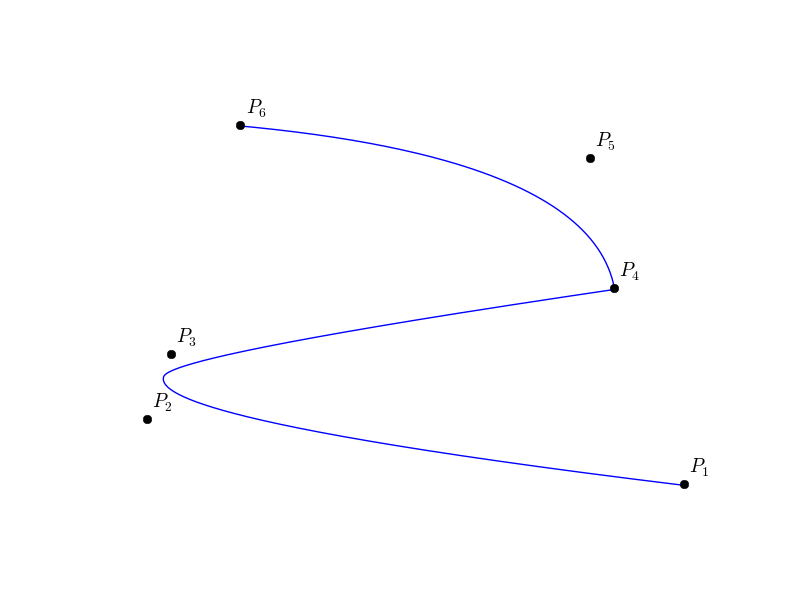
\includegraphics[width=9cm,height=9cm]{\RepFigures/courbe_bsplines.png} &
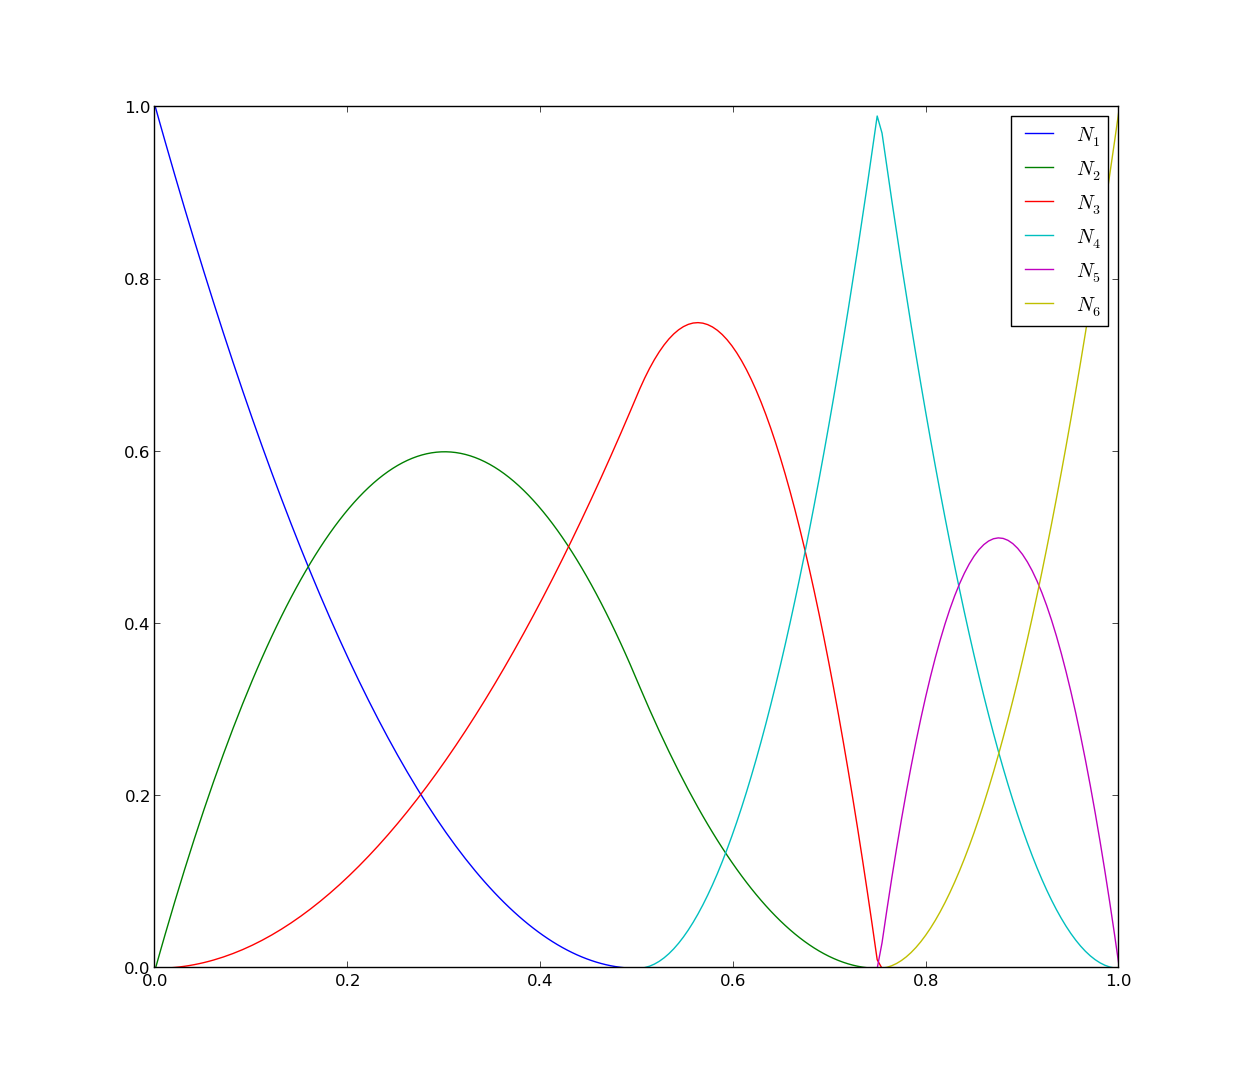
\includegraphics[width=8cm,height=8cm]{\RepFigures/basis_fct_p2_N5.png} 
\end{tabular}
\caption{(left) A quadratic B-Spline curve and its control points using the knot vector $T = \{ 000~  \frac{1}{2}~ \frac{3}{4} \frac{3}{4}~ 1 1 1 \}$, (right) the corresponding B-Splines.}
\label{figBSplineCurve}
\end{center}
\end{figure}


%\subsection{B-splines curves properties}
We have the following properties for a \textit{B-spline} curve:
\begin{itemize}
\item If $n=k$, then $\mathcal{C}$ is just a B\'ezier-curve,
\item $\mathcal{C}$ is a piecewise polynomial curve,
\item The curve interpolates its extremas if the associated multiplicity of the first and the last knot are maximum (\textit{i.e.} equal to $k$), \textit{i.e.} open knot vector,
\item Invariance with respect to affine transformations,
\item Strong convex-hull property:

if $t_i \leq t \leq t_{i+1}$, then $\mathcal{C}(t)$ is inside the convex-hull associated to the control points $\mathbf{P}_{i-p},\cdots,\mathbf{P}_{i}$,

\item Local modification : moving the $i^{th}$ control point $\mathbf{P}_{i}$ affects $\mathcal{C}(t)$, only in the interval $[t_i,t_{i+k}]$,
\item The control polygon approaches the behavior of the curve.
\end{itemize}
\begin{remark} 
In order to model a singular curve, we can use multiple control points : $\mathbf{P}_{i}=\mathbf{P}_{i+1}$.
\end{remark}

\subsection{Fundamental geometric operations }
By inserting new knots into the knot vector, we add new control points without changing the shape of the B-Spline curve. This can be done using the DeBoor algorithm \cite{DeBoor_Book2001}. We can also elevate the degree of the B-Spline family and keep unchanged the curve \cite{qi}. In (Fig. \ref{refinement_curve_B_Spline}), we apply these algorithms on a quadratic B-Spline curve and we show the position of the new control points.  
\\
\paragraph{Knot insertion.}~
\label{subsubsec:knot_insert}
After modification, we denote by $\widetilde{n}, \widetilde{k}, \widetilde{T} $ the new parameters. $(\textbf{Q}_i)$ are the new control points.
\\
One can insert a new knot $t$, where $ t_j \leqslant t < t_{j+1}$. For this purpose we use the DeBoor algorithm \cite{DeBoor_Book2001}:
$$\widetilde{n} = n+1$$
$$\widetilde{k} = k$$
$$ \widetilde{T} = \{ t_1,.., t_j, t, t_{j+1},.., t_{n+k}\}$$
$$
\alpha_i = \left\{\begin{array}{cc}1 & 1 \leqslant i \leqslant j-k+1 \\\frac{t-t_i}{t_{i+k-1}-t_i} & j-k+2 \leqslant i \leqslant j \\0 & j+1 \leqslant i \end{array}\right. 
$$
$$
\textbf{Q}_i = \alpha_i \textbf{P}_i + (1-\alpha_i) \textbf{P}_{i-1}
$$   
Many other algorithms exist, like blossoming for fast insertion algorithm. For more details about this topic, we refer to \cite{goldman_lyche_book}. 
% TODO : inserer figures d'exemple d'insertion de noeuds
%\subsubsection{Order elevation}
%We can elevate the order of the basis, without changing the curve. Several algorithms exist for this purpose. We used the one by Huang et al. \cite{prautzsch,qi}:


\todo{TODO: figure a refaire avec les points de controle affiches}
%
\begin{figure}[!ht]
\begin{center}
\begin{tabular}{cc}
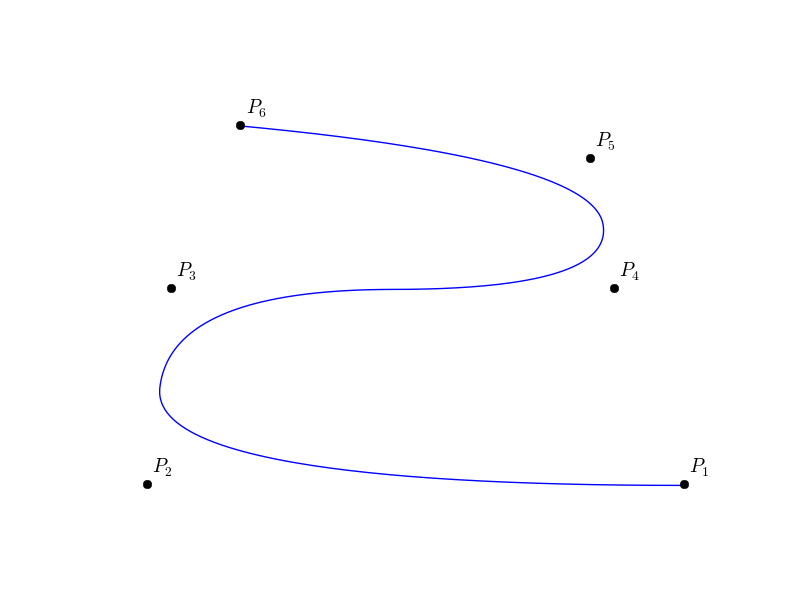
\includegraphics[width=8cm,height=8cm]{\RepFigures/curve} &
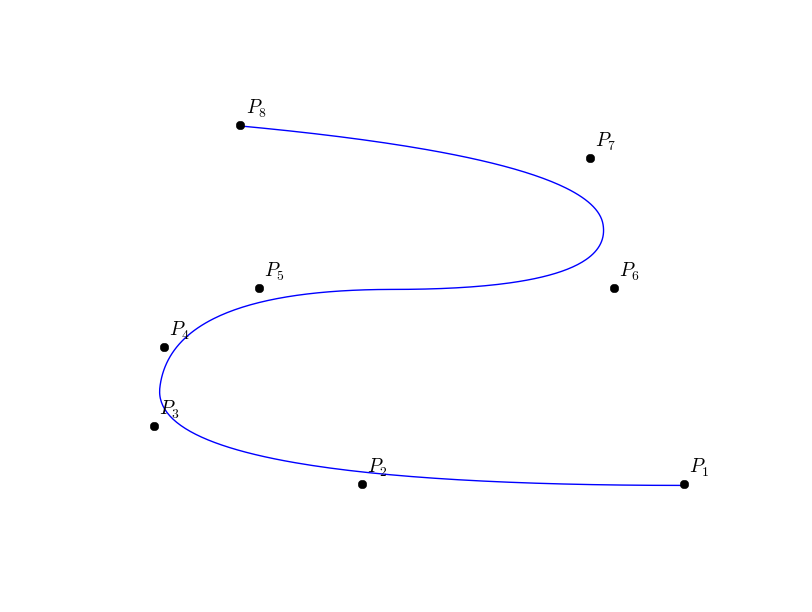
\includegraphics[width=8cm,height=8cm]{\RepFigures/curve_p0_n9} 
\\
(a) & (b)
\\
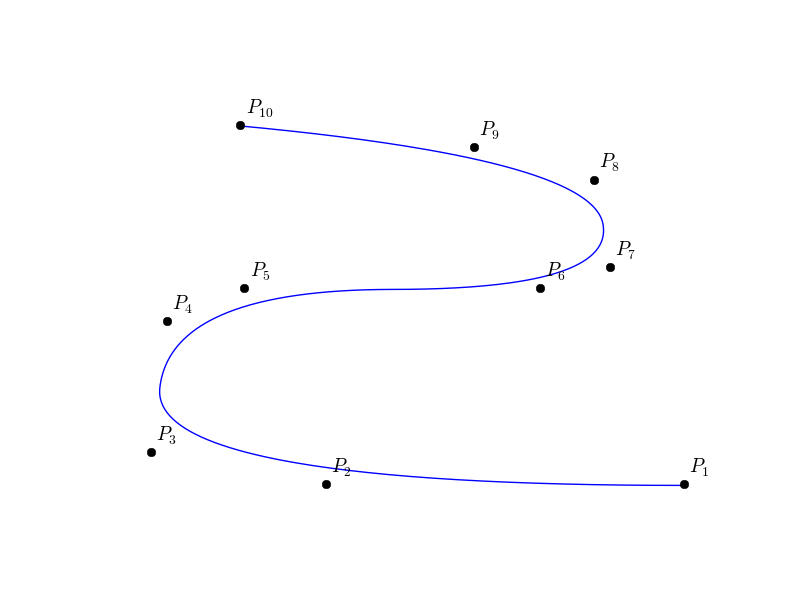
\includegraphics[width=8cm,height=8cm]{\RepFigures/curve_p2_n0} &
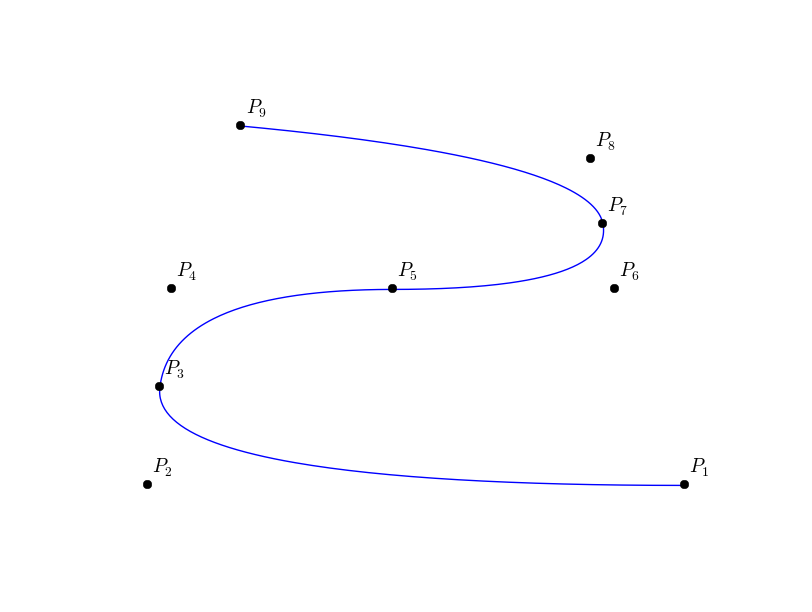
\includegraphics[width=8cm,height=8cm]{\RepFigures/curve_p0_n3_bezier}
\\
(c) & (d)
\end{tabular}
\caption{(a) A quadratic B-spline curve and its control points. The knot vector is $T = \{ 000, \frac{1}{4}, \frac{1}{2}, \frac{3}{4}, 1 1 1 \}$. 
(b) The curve after a h-refinement by inserting the knots $\{ 0.15, 0.35\}$ while the degree is kept equal to $2$. 
(c) The curve after a p-refinement, the degree was raised by $1$ (using cubic B-splines). 
(d) The curve after duplicating the multiplicity of the internal knots $\{ \frac{1}{4}, \frac{1}{2}, \frac{3}{4} \}$, 
this leads to a B\'ezier description. We can then, split the curve into $4$ pieces (sub-domains), each one will corresponds to a quadratic B\'ezier curve.}
\label{refinement_curve_B_Spline}
\end{center}
\end{figure}

\subsection{Deriving a B-spline curve} 
\label{subDerivCurve}
The derivative of a B-spline curve is obtained as:
\begin{equation}
\mathcal{C}^{\prime}(t) = \sum_{i=1}^{n} {N_{i}^{k}}^{\prime}(t) \mathbf{P}_i = \sum_{i=1}^{n} \left(\frac{p}{t_{i+p}-t_{i}}N_{i}^{k-1}(t) \mathbf{P}_i - \frac{p}{t_{i+1+p}-t_{i+1}}N_{i+1}^{k-1}(t) \mathbf{P}_i \right)
= \sum_{i=1}^{n-1} {N_{i}^{k-1}}^{\ast}(t) \mathbf{Q}_i
\end{equation}
where $\mathbf{Q}_i = p \frac{\mathbf{P}_{i+1} - \mathbf{P}_i}{t_{i+1+p}-t_{i+1}}$, and $\{{N_{i}^{k-1}}^{\ast},~~1 \leq i \leq n-1\}$ are generated using the knot vector $T^{\ast}$ % = \{ 0\cdots 0, \cdots \cdots, 1\cdots 1 \}$, 
which is obtained from $T$ by reducing by one the multiplicity of the first and the last knot (in the case of open knot vector), \textit{i.e.} by removing the first and the last knot.
\\
More generally, by introducing the B-splines family $\{ {N_{i}^{k-j}}^{\ast}, 1 \leq i \leq n-j \}$ generated by the knots vector $T^{j^{\ast}}$ obtained from $T$ by removing the first and the last knot $j$ times, we have the following result:
\begin{proposition} The $j^{th}$ derivative of the curve $\mathcal{C}$ is given by
$$
\mathcal{C}^{(j)}(t) = \sum_{i=1}^{n-j} {N_{i}^{k-j}}^{\ast}(t) \mathbf{P}_i^{(j)}
$$
where, for $j>0$,
$$
\mathbf{P}_i^{(j)} = \frac{p-j+1}{t_{i+p+1}-t_{i+j}} \left( \mathbf{P}_{i+1}^{(j-1)} - \mathbf{P}_i^{(j-1)} \right)
$$
and $\mathbf{P}_i^{(0)} = \mathbf{P}_i$.
\end{proposition}
By denoting $\mathcal{C}^{\prime}$ and $\mathcal{C}^{\prime\prime}$ the first and second derivative of the B-spline curve $\mathcal{C}$, it is easy to show that:
\begin{proposition}
We have,
\begin{itemize}
 \item $\mathcal{C}^{\prime}(0) = \frac{p}{t_{p+2}} \left(\mathbf{P}_{2} - \mathbf{P}_1\right)$,
 \item $\mathcal{C}^{\prime}(1) = \frac{p}{1-t_{n}} \left(\mathbf{P}_{n} - \mathbf{P}_{n-1}\right)$,
 \item $\mathcal{C}^{\prime\prime}(0) = \frac{p(p-1)}{t_{p+2}} \left( \frac{1}{t_{p+2}}\mathbf{P}_{1} 
- \{ \frac{1}{t_{p+2}} + \frac{1}{t_{p+3}} \} \mathbf{P}_2 + \frac{1}{t_{p+3}}\mathbf{P}_{3} \right)$,
 \item $\mathcal{C}^{\prime\prime}(1) = \frac{p(p-1)}{1-t_{n}} \left( \frac{1}{1-t_{n}}\mathbf{P}_{n} 
- \{ \frac{1}{1-t_{n}} + \frac{1}{1-t_{n-1}} \} \mathbf{P}_{n-1} + \frac{1}{1-t_{n-1}}\mathbf{P}_{n-2} \right)$.
\end{itemize}
\end{proposition}
%TODO diagramme a inserer : mettre accolade pour montrer la multiplicte des noeuds extremaux qui passe a k-1 au lieu de k
\paragraph{Example:} 
Let us consider the quadratic B-spline curve associated to the knots vector $T=\{000~\frac{2}{5}~\frac{3}{5}~111 \}$ and the control points $\{ P_i, 1 \leq i \leq 5 \}$:

$$
\mathcal{C}(t) = \sum_{i=1}^{5} {N_{i}^{3}}^{\prime}(t) \mathbf{P}_i 
$$
we have, 
$$
\mathcal{C}^{\prime}(t) = \sum_{i=1}^{4} {N_{i}^{2}}^{\ast}(t) \mathbf{Q}_i
$$
where 
$$
\mathbf{Q}_1 = 5 \{\mathbf{P}_{2} - \mathbf{P}_1\}, ~~~~\mathbf{Q}_2 = \frac{10}{3} \{ \mathbf{P}_{3} - \mathbf{P}_2\},
$$
$$
\mathbf{Q}_3 = \frac{10}{3} \{ \mathbf{P}_{4} - \mathbf{P}_3\},~~~~\mathbf{Q}_4 = 5 \{\mathbf{P}_{5} - \mathbf{P}_4\}.
$$
The \textit{B-splines} $\{ {N_{i}^{2}}^{\ast},~~1 \leq i \leq 4\}$ are associated to the knot vector $T^{\ast}=\{00~\frac{2}{5}~\frac{3}{5}~11 \}$. 

\subsection{Intersection of two spline curves}
\todo{TODO}

\subsection{Multivariate tensor product splines}
Let us consider $d$ knot vectors $ \mathcal{T} = \{T^1,T^2,\cdots,T^d\}$. For simplicity, we consider that these knot vectors are open, which means that $k$ knots on each side are duplicated so that the spline is interpolating on the boundary, and of bounds $0$ and $1$. In the sequel we will use the notation $I=[0,1]$.
Each knot vector $T^i$, will generate a basis for a Schoenberg space, $\mathcal{S}_{k_{i}}(T^i,I)$. The tensor product of all these spaces is also a Schoenberg space, namely $\mathcal{S}_{\mathbf{k}}(\mathcal{T})$, where $\mathbf{k}=\{k_1,\cdots,k_d\}$. The cube $\mathcal{P}=I^d=[0,1]^d$, will be referred to as a patch.
\\
The basis for $\mathcal{S}_{\mathbf{k}}(\mathcal{T})$ is defined by a tensor product :
$$
N_{\mathbf{i}}^{\mathbf{k}} := N_{i_1}^{k_1} \otimes N_{i_2}^{k_2} \otimes \cdots \otimes N_{i_d}^{k_d}
$$
where, $\mathbf{i}=\{i_1,\cdots , i_d \}$.
\\
A typical cell from $\mathcal{P}$ is a cube of the form : $Q_{\mathbf{i}}=[\xi_{i_1}, \xi_{i_1+1}] \otimes \cdots \otimes [\xi_{i_d}, \xi_{i_d+1}]$. %To any cell $Q$, we will associate its extension $\widetilde{Q}$, which is the union of the supports of basis functions, that intersects $Q$.
